% !TeX root = ../main.tex
% Add the above to each chapter to make compiling the PDF easier in some editors.

\chapter{Sioux Falls Network Calibration}\label{chapter:sioux_falls_network_calibration}
The second part of the project consists on calibrating a smaller city network using a traffic simulator. In this case, the Sioux Falls network has been used together with SUMO (Simulation of Urban MObility) for microscopic and continuous road traffic simulation.

\section{Minimum required simulation runs}
\subsection{Intuition behind}
SUMO provides the capability to simulate traffic conditions on a given network. In order to obtain meaningful results while calibrating the network, multiple simulations counts of the network detectors are required. Since every SUMO simulation might require a good amount of time to complete, specially for bigger networks (Munich, for example), a minimum number of simulation runs that still provide statistically significant results can be obtained. As seen during the lecture, the formula to obtain this value is given as:

\begin{equation}
  \boldsymbol{n} = \cfrac{2^2 * t_{(1-\alpha/2, N - 1)} * S^2}{CI^2}; N \geq n
  \label{eq:21}
\end{equation}

where N is the number of runs executed, n is the minimum number of runs required, S is the standard deviation calculated from prior simulation runs (for few detectors with the highest traffic flows), CI is the confidence interval given as \((1 - \alpha) * \mu\), \(\alpha\) is the confidence level and t is the student's t statistic. 

\subsection{Code implementation}
In order to calculate the number of simulation runs required, the following code has been used on the counts obtained from SUMO:

\lstinputlisting{figures/simulationRuns.m}

After the N simulation runs were executed, the formula has been applied for every detector in the results to obtain the minimum simulation runs. After a couple of trials, 13 happened to be a good value for the number of simulation runs required to obtain statistically significant results, satisfying the condition \(N \geq n\). Table \ref{tab:simulation-runs} shows some the outputs obtained when using 13 as number of simulation runs.

\begin{table}[htpb]
  \centering
  \begin{tabular}{l l l l l l}
    \toprule
      N & S & $\mu$ & CI & t & n \\
    \midrule
      13 & 2.574 & 68.94 & 3.44 & 2.178 & 10.59  \\
      13 & 1.687 & 70.53 & 3.52 & 2.178 & 4.34  \\
      13 & 2.043 & 69.25 & 3.46 & 2.178 & 6.61  \\
      13 & 2.466 & 70.51 & 3.52 & 2.178 & 9.29  \\
      13 & 1.757 & 70.12 & 3.50 & 2.178 & 4.76  \\
    \bottomrule
  \end{tabular}
  \caption[Minimum SUMO Simulation Runs]{Required SUMO simulation runs}
  \label{tab:simulation-runs}
\end{table}

\section{Network calibration}
Using the previous results for the number of simulation runs, the Sioux Falls network has been calibrated. Also, as seen during the lecture, 10 is the rule of thumb value while choosing the number of simulation runs required for obtaining statistically significant results.SUMO provides two different simulation modes: dynamic user equilibrium (DUA) and trip-based. Both modes have been used to calibrate the network using SPSA as approximation method. The results of both calibrations are further compared and an analysis of the two simulation methods is provided at the end. 

\subsection{DUAiterate calibration}
After tuning the SPSA parameters with 6 different configurations, the parameters shown in table \ref{tab:calibration-params-sf-dua} provided the best results among them, shown in table \ref{tab:top3-rmsn-sf-dua}. Also, the worst 3 results for the RMSN obtained during the calibration are shown in table \ref{tab:top3-rmsn-sf-dua}.

\begin{table}[htpb]
  \centering
  \begin{tabular}{l l l l l l l l l}
    \toprule
      - & a & c & A & Alpha & Gamma & G & N & seg\\
    \midrule
      SPSA & 30 & 3 & 50 & .4 & .2 & 3 & 40 & 6 \\
    \bottomrule
  \end{tabular}
  \caption[Calibration Parameters SF DUA]{Calibration parameters for Sioux Falls DUA calibration}
  \label{tab:calibration-params-sf-dua}
\end{table}
\begin{table}[htpb]
  \centering
  \begin{tabular}{l l}
    \toprule
      Top 3 & Worst 3 \\
    \midrule
      .2191 & .5863 \\
      .2235 & .4184 \\
      .2249 & .3901 \\
    \bottomrule
  \end{tabular}
  \caption[Top Worst 3 RMSN SF DUA]{Top and worst 3 RMSN values for Sioux Falls DUA calibration}
  \label{tab:top3-rmsn-sf-dua}
\end{table}

\subsection{Trip-based calibration}
After tuning the SPSA parameters with 6 different configurations, the parameters shown in table \ref{tab:calibration-params-sf-dua} provided the best results among them, shown in table \ref{tab:top3-rmsn-sf-dua}. Also, the worst 3 results for the RMSN obtained during the calibration are shown in table \ref{tab:top3-rmsn-sf-dua}. Compared to DUAiterate, only the c parameter varied for the trip-based calibration.

\begin{table}[htpb]
  \centering
  \begin{tabular}{l l l l l l l l l}
    \toprule
      - & a & c & A & Alpha & Gamma & G & N & seg\\
    \midrule
      SPSA & 30 & 9 & 50 & .4 & .2 & 3 & 40 & 6 \\
    \bottomrule
  \end{tabular}
  \caption[Calibration Parameters SF DUA]{Calibration parameters for Sioux Falls DUA calibration}
  \label{tab:calibration-params-sf-dua}
\end{table}
\begin{table}[htpb]
  \centering
  \begin{tabular}{l l}
    \toprule
      Top 3 & Worst 3 \\
    \midrule
      .3291 & .9209 \\
      .3472 & .6895 \\
      .3611 & .6812 \\
    \bottomrule
  \end{tabular}
  \caption[Top Worst 3 RMSN SF trip]{Top and worst 3 RMSN values for Sioux Falls trip-based calibration}
  \label{tab:top3-rmsn-sf-dua}
\end{table}
\subsection{Comparing results}
DUAiterate provides better results because when the simulation starts, it is already iterating (iteration fixed to 4 in the code) to achieve user equilibrium. In traffic assignment, this means that the network is at equilibrium condition when all drivers have selected routes that minimize their travel time. The route choice in DUAiterate is therefore closer to the final traffic assignment, thus yielding to better results. On the other hand, trip-based is just a one-shot assignment to the shortest path at the time of vehicle departure. This causes the traffic assignment to be more distant from the optimum.

\begin{figure}[htpb]
  \centering
  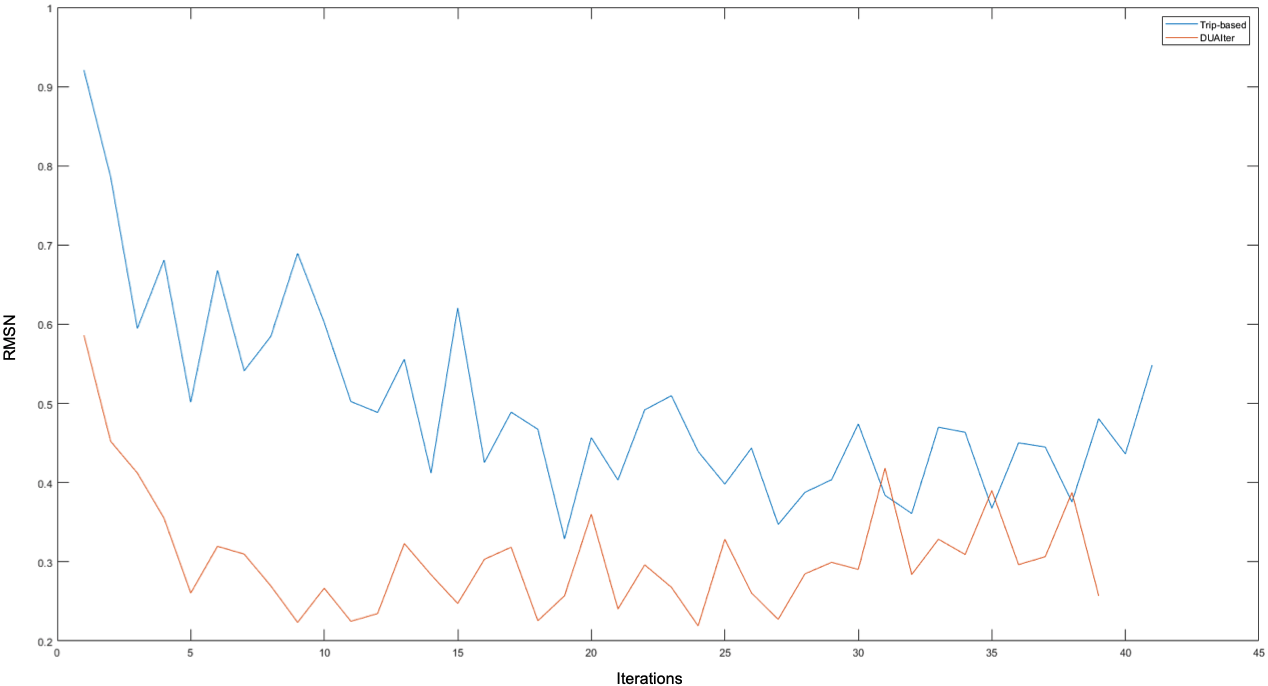
\includegraphics[width=0.6\textwidth]{figures/dua-trip-comparison.png}
  \caption{Results comparison of DUAiterate calibration vs trip-based calibration}
  \label{fig:dua-vs-trip-sf}
\end{figure}

\subsection{Remarks and challenges}
Along the process of calibrating the Sioux Falls network using SPSA, the following challenges and tasks where encountered/performed: 

\begin{itemize}
  \item Code modified in order to avoid repeating operations to improve speed (+-ve perturbations).
  \item Preallocation of matrices and variables to improve speed within SPSA operation.
  \item Improvements helped to reduce calibration time around 10\% (more notorious while calibrating Munich Network).
  \item Created gitlab repository (LRZ) to track file versions, changes and results. 
  \item Issues with dlr.sumo.de. Used local documentation instead.
\end{itemize}
